\subsection{Esecuzione dell'esperienza}

La prima operazione fatta è stata quella di verificare il corretto allineamento dell'interferometro. Abbiamo infatti notato che se i due specchi non sono perpendicolari tra loro, sullo schermo si vedono figure di interferenza complicate e difficili da trattare invece che una semplice figura di interferenza lineare in cui si alternano massimi e minimi. Per allineare lo strumento è sufficiente ruotare delicatamente i due specchi finche non compare sullo schermo una figura d'interferenza semplice.

%Facciamo notare che nonostante l'attenzione prestata, lo specchio e lo schermo non sono risultati essere perfettamente paralleli tra di loro. Questo comporta che i due raggi luminosi incidenti sullo schermo non sono allineati tra di loro. Infatti sullo schermo si visualizzano in alternanza delle frange di interferenza costruttiva e distruttiva, ovvero picchi luminosi e non che si alternano con regolarità.
% WTF????

La misura dell'indice di rifrazione di un dato materiale con l'interferometro di Michelson si esegue adottando la seguente strategia.
Si parte da una configurazione base, per esempio l'interferometro con un ramo su cui e già stata montata la camera da vuoto
(si veda la Figura \ref{fig:mik}). A questo punto sullo schermo è proiettata una figura di interferenza. Dopodiché si
varia gradualmente un qualche parametro del materiale sotto esame, per esempio: la pressione (nel caso dell'aria), la lunghezza,
l'inclinazione oppure la concentrazione (per una soluzione). Questo serve per variare il cammino ottico del raggio che attraversa il materiale.
In questo modo la figura di interferenza varia e le frange si muovono. La seguente relazione lega il numero $N$ di frange passate sullo schermo,
alla differenza di cammino ottico $d$.

\begin{equation}
    N \,=\, \frac{d}{\lambda} = \frac{\Delta n \cdot 2 \ell}{\lambda}
\end{equation}
%
Nella formula $\lambda$ indica la lunghezza d'onda della luce, $\Delta n$ la differenza di indice di rifrazione tra la configurazione base
e quella attuale, mentre $2\ell$ e la lunghezza della camera (il 2 serve perché la luce attraversa la camera due volte).

Una volta giunti al valore di pressione, lunghezza concentrazione voluto,


\begin{SCfigure}[0.70][t]
    \centering
    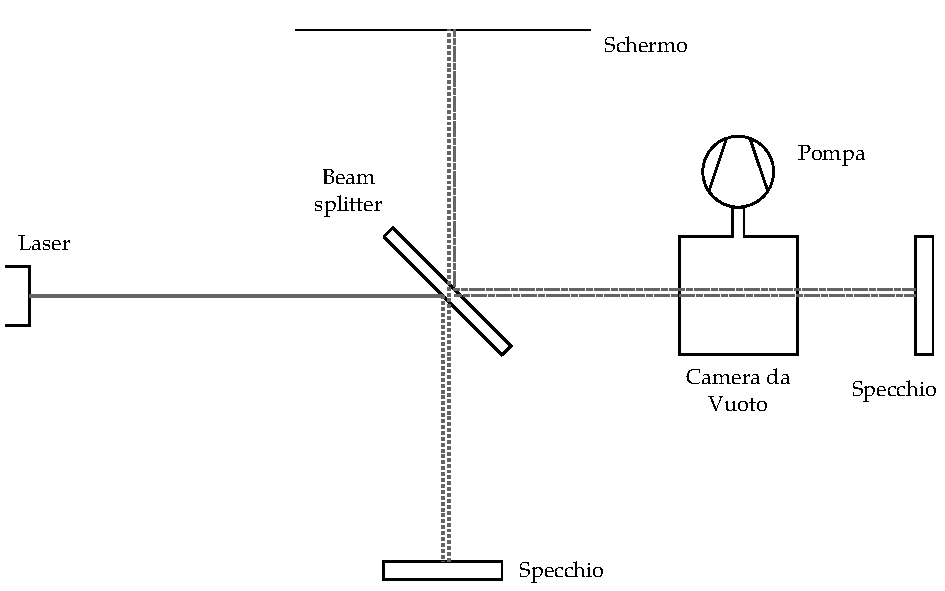
\includegraphics[width=120mm]{drawing.pdf}
    \caption{Schema semplificato del sistema utilizzato per misurare l'indice di rifrazione dell'aria.}
    \label{fig:mik}
\end{SCfigure}

\subsubsection{Indice di rifrazione dell'aria}

Detto questo la procedura eseguita per ricavare l'indice di rifrazione dell'aria è la seguente:

\begin{itemize}
	\item{Abbiamo installato sul sistema, tra il beam splitter e lo specchio mobile, una piccola camera da vuoto con due pareti in vetro atte a far passare la luce. La camera è stata collegata, mediante la valvola a spillo alla pompa a membrana;} %Infatti variando la pressione dell'aria interna alla camera da vuoto si varia l'indice di rifrazione di quest'ultima. Pertanto il cammino ottico compiuto dal raggio lumnoso riflesso risulta essere differente da quello del raggio luminoso rifratto;}
    \item{Partendo con la camera da vuoto a pressione atmosferica abbiamo man mano creato il vuoto all'interno della camera regolando l'apertura della valvola a spillo. Aprendo la valvola a spillo (ovviamente con la pompa accesa), l'aria esce dalla camera da vuoto e viene pompata fuori;}
    \item{Ad intervalli regolari di pressione, ovvero ogni \SI{10}{\kilo\pascal}, abbiamo annotato il numero di frange di interferenza passate sullo schermo;}
\end{itemize}

\subsubsection{Indice di rifrazione del vetro}

Per misurare l'indice di rifrazione del vetro abbiamo adottato una strategia simile. Dobbiamo partire da una data figura di interferenza e variare il cammino ottico di uno dei due raggi. Poi dobbiamo contare il numero di massimi di intensità (ovvero dei punti )

\subsection{Analisi Dati}

Per ricavare l'indice di rifrazione dell'aria abbiamo sfruttato la legge fisica che ci dice che:

Ricordiamo che a condizione di pressione costante il cammino ottico percorso dai due raggi luminosi risulta essere lo stesso.
Quindi lo scopo sarà quello di confrontare il numero di frange contate con la differenza di pressione rilevata. Infatti variando la pressione nella camera da vuoto si varia l'indice di rifrazione dell'aria. Questo provoca una variazione nel cammino ottico del raggio riflesso dallo specchio semitrasparente e quindi fenomeni di diffrazione che saranno sempre più accentuati man mano che l'indice di rifrazione dell'aria varia infunzione della pressione interna alla camera. buzz culo !!!!
Sapendo che il cammino ottico è pari a due volte la lunghezza della camera da vuoto moltiplicata per lindice di rifrazione del gas ivi contenuto ...
